\section{Genetic Algorithm}
\label{sec:genetic}
\vspace{-0.45cm}
Genetic algorithms are search algorithms based on the mechanics of natural selection and genetics as observed in the biological world. They use both, “survival of the fittest” and "mutation" (randomization) to robustly explore the best choice of weights.

%\subsection{Pipeline}
%Diagram of the genetic algorithm architecture and description how the code runs 
\vspace{-0.4cm}
\subsection{Features}
To determine the next move, all possible move are compared using a utility function and the move resulting in the highest utility is chosen. The utility function is a weighted sum of different, state-dependent, human engineered features. A "good" choice of features therefore is crucial in order to obtain a well-performing agent.
\newline 
The current state is defined by the occupancy of the board and the next Tetramino. One can also define abstract state descriptors like the height of columns, holes, wells and transitions. A hole is an empty cell with an occupied cell above it. A well is a column whose adjacent columns are higher than it, and its depth is defined as the difference of the height of well column and the shorter adjacent column. Transitions are the number of empty-occupied cell switches in the respective column or row. The final set of features we used are: 

\begin{enumerate}
\itemsep0em 
\item Sum of height differences between adjacent columns.
\item Maximum height of a column.
\item Total number of cleared rows.
\item Whether the current move results in a loss.
\item Total number of holes. 
\item Sum of depths of all wells in the game board.
\item Mean of the absolute difference between the height of each column and the mean height
\end{enumerate}
\vspace{-0.45cm}
%Initial state, crossing over and mutations
\subsection{Training Algorithm Implementation}
In order to find an optimal set of weights, several steps are repeated iteratively: First, an initial population of randomly drawn weight vectors from a uniform(0, 1) distribution is generated. 
\newline
To produce the subsequent generations, we first choose a parent in the following way: We calculate the sum of scores of all members of the previous generation and multiply it with a random number from a uniform(0,1) distribution to define a threshold value. We then randomly draw members from the previous generation and check if their score crosses the threshold value. If it does, we choose that member as as a parent. Else we reduce this threshold and continue the search by drawing a different member from the population. In case no member of the previous generation crosses the threshold, we return the member with the highest score in the previous generation as the parent.
\newline
After selection two parents using the above method, we use the single point crossing over heuristic to determine the weights of the two children produced. In this heuristic, a single crossover point on both parents' weight sequence is selected. All weights beyond that point in the parents' weight sequence is swapped between the two parent organisms to generate the two children. We used a 0.6\% crossing-over rate. The rate defines the probability for the crossing over to happen. In case crossing over does not happen, the parents chosen are directly passed as children to the next generation.

Subsequently, each weight of the child can undergo mutation with 1\% probability. If a mutation occurs, the specific weight is multiplied with a uniformly drawn value between 0.8 and 1.2.

\subsection{Parallel Processing}
Due to the randomness in the choice of next stone, each game is different. In order to avoid "overfitting", i.e. a set of weights merely performs well for a specific sequence of stones, the score for each member is the average score of 10 games. As these games are independent from each other, they are played in parallel, using multi-threading. Similarly, each member of the population has its own set of independent feature weights and hence, they are also evaluated leveraging multi-threading.
This achieves a speedup of roughly 10.82, e.g. given a population size of 50, the multi-threaded version needs \texttt{7m53s} per generation while the older version needed \texttt{85m19s}.

\subsection{Results}
We analyze the results from 100 runs of the game using the weight vector $\vec{w}$ shown right below, which were derived training our best genetic algorithm for 200 generations with a population size of 40. The weights of the features are ordered as in Section 2.1. 

$$\vec{w} = 
\begin{bmatrix}
0.69, -0.60, 0.80, 1.07, 0.68, 1.13, 3.63
\end{bmatrix}$$

Figure \ref{fig:graph_100_runs} gives us the distribution of the performance results from 100 iterations. We observe that while most results are below 100,000 rows cleared, there are 10 iterations where we clear more than 200,000 rows.  

\centering
\begin{tabular}{| l | c |}
\hline
\textbf{Metric} & \textbf{Value} \\
\       hline
Average & 119,560 	\\ \hline
Median & 82,706 		\\ \hline
Maximum & 864,157 		\\ \hline
Minimum & 101		 	\\ \hline
\end{tabular}
\captionof{table}{Performance of best weights over 100 iterations}
\justify

Table 2 shows us that the while the minimum number of rows cleared is 101, we clear a maximum of 864,157 rows. The average number of rows cleared is 119,560 which is cleary higher than the median of 82,706. This aberration is due to our extremely well performing runs when the sequence of incoming stones is very beneficial to our set of weights.

Figure \ref{fig:mean_median_graph} shows that there is a linear relationship between the mean and the median of the 10 best results of each generation during training. This means that we don't get random outliers of weights which give good scores for very few members while all others perform poorly. Instead we have a smooth development and increase of the performance during training. Also, the graph shows that the mean scores during training are lower for population sizes of 15 and 25, and increases significantly for population sizes greater than 40. The performance tends to converge for population size 40, as there isn't any improvement with population size 100. This means that the population size has to pass a certain threshold such that the random processes of crossing over and mutation are likely to "produce" significant improvements.

\begin{Figure}
\centering
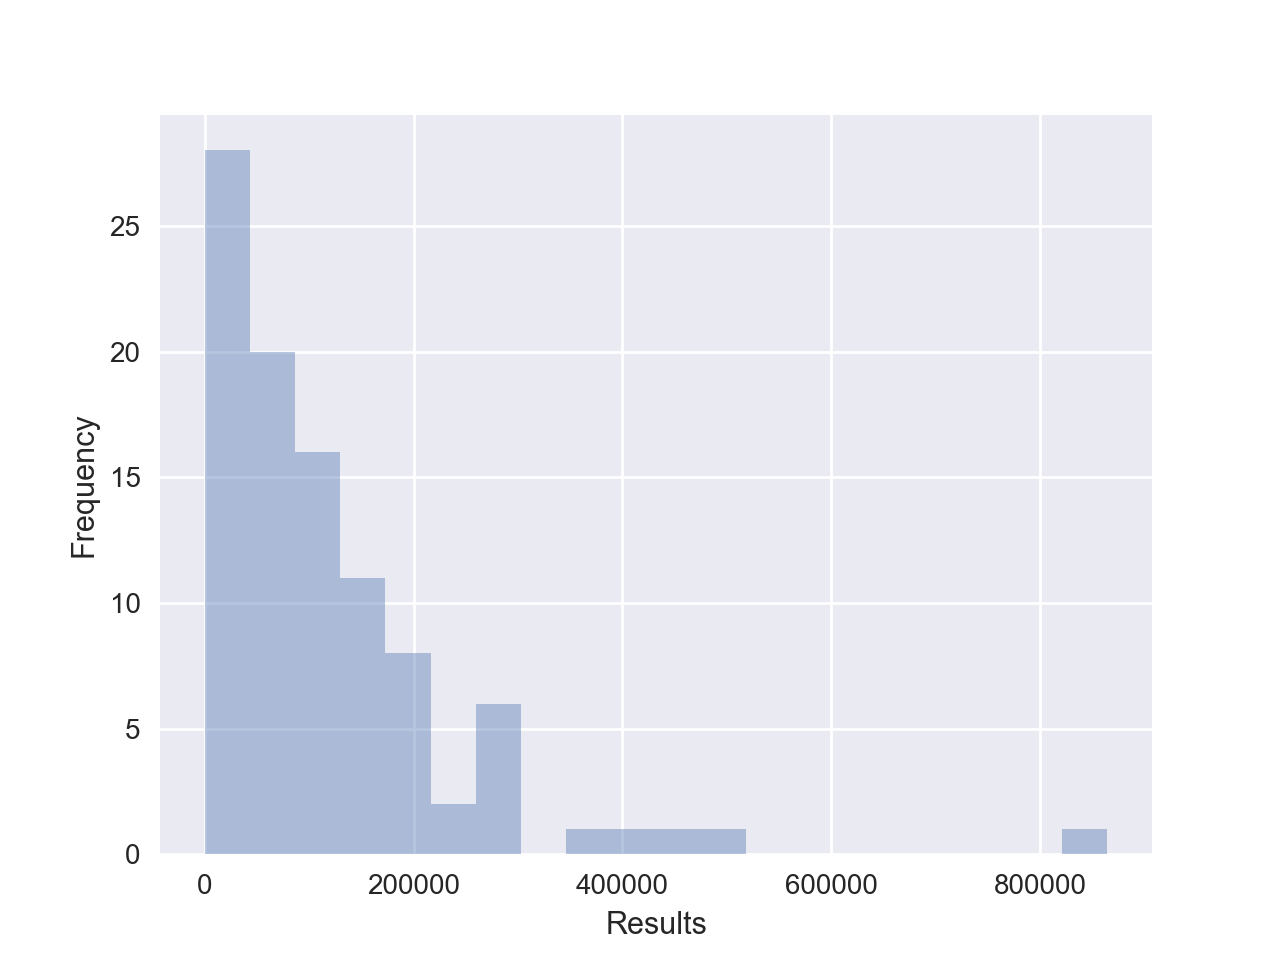
\includegraphics[width=8cm]{imgs/Results_Hists.png}
\captionof{figure}{Results from 100 iterations of the game}
\label{fig:graph_100_runs}
\end{Figure}

\begin{Figure}
\centering
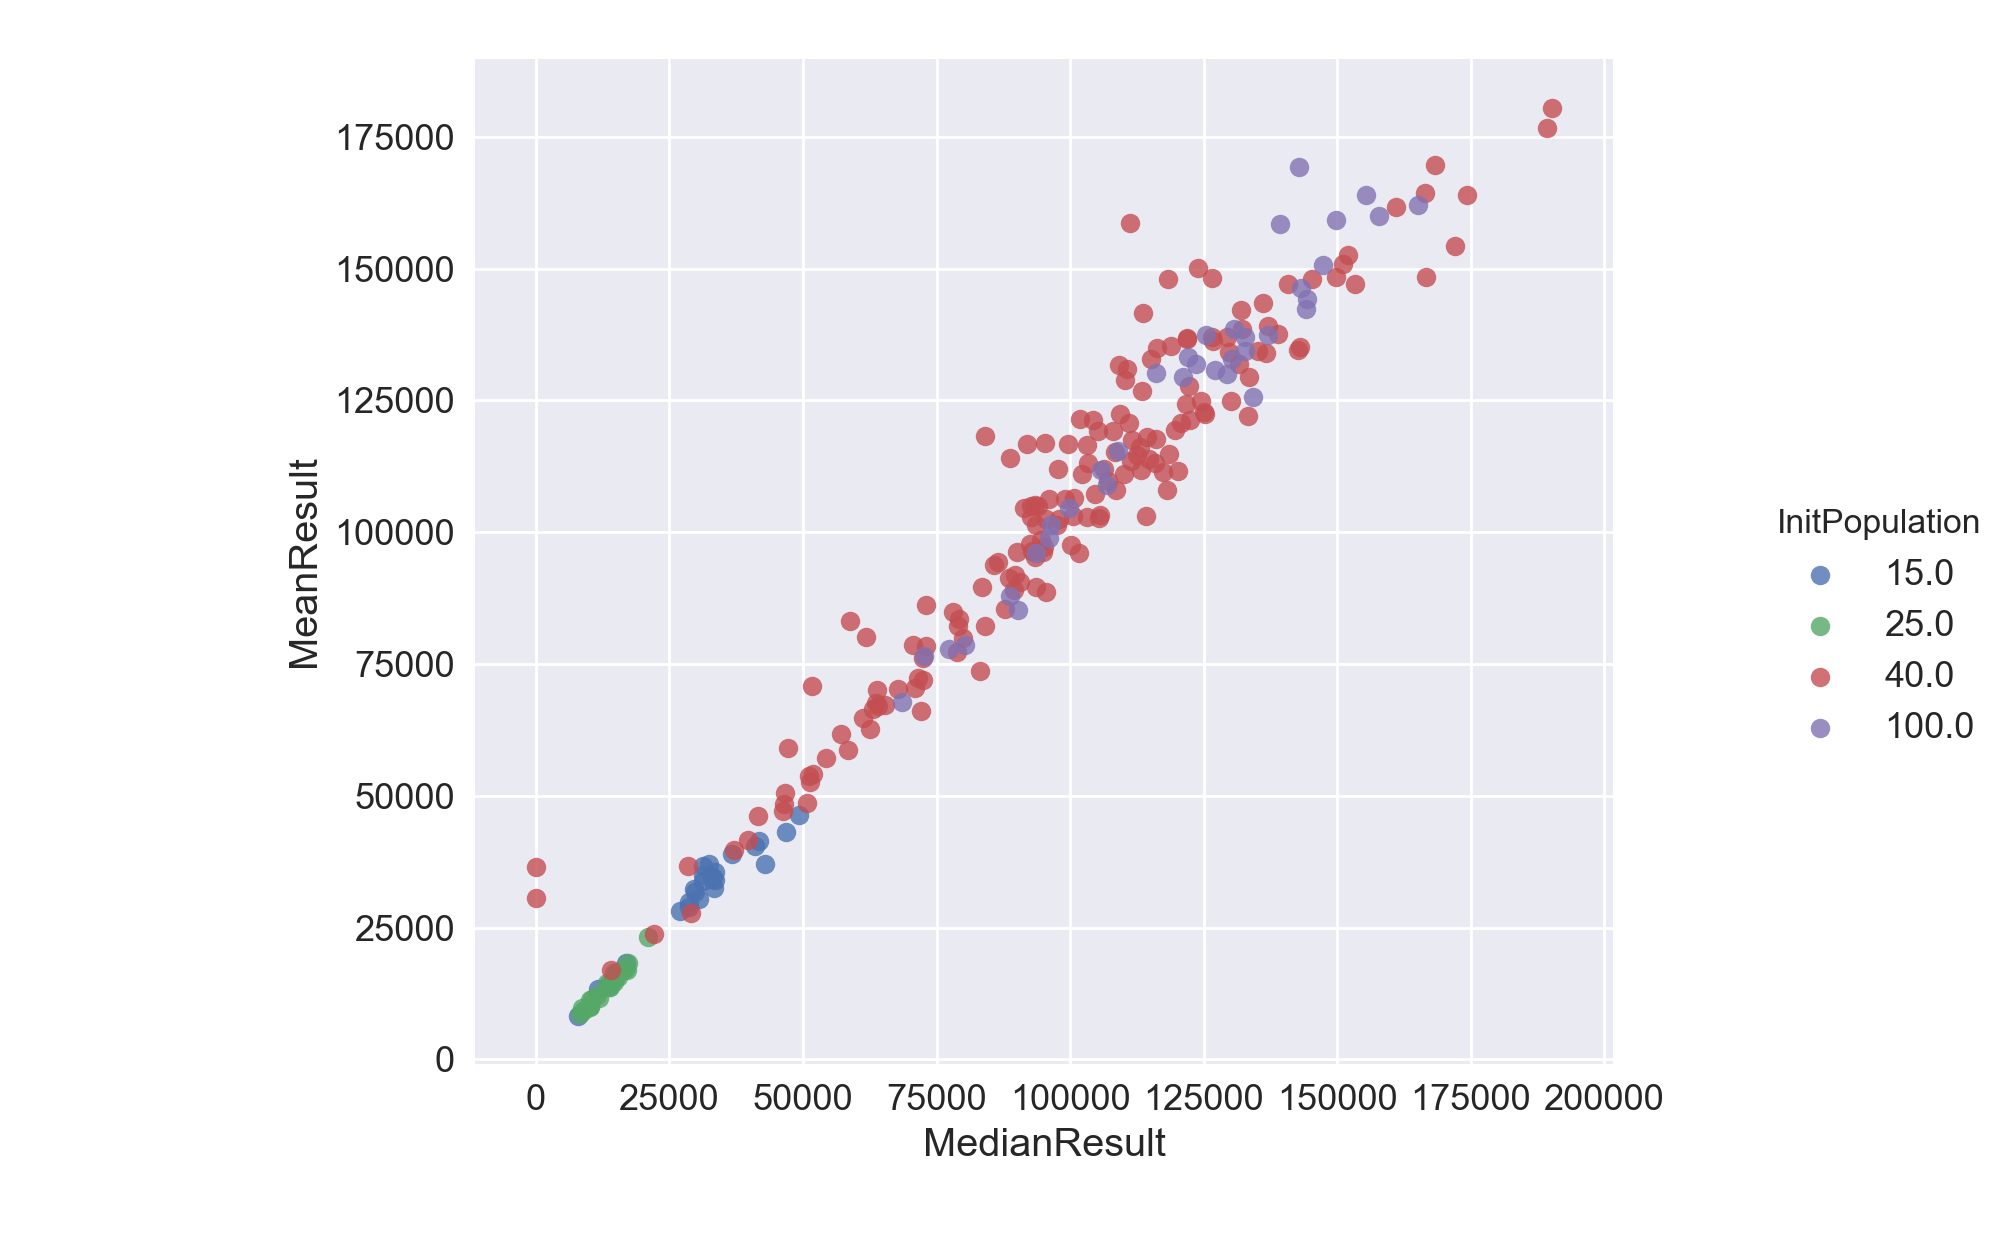
\includegraphics[width=8cm]{imgs/Median_Mean.png}
\captionof{figure}{Mean-Median plot of intermediate scores during training for different population sizes.}
\label{fig:mean_median_graph}
\end{Figure}

% \subsection{Analysis}
% W
% ...\textit{Which performs best ?}

% Maybe we can say that we don't have amazing results because we didn't train it enough since we thought that there was a problem in our approach. We thought that because of the results of others (cite other papers) 